\chapter{Test problems}
\begin{overview}
To verify that the system is working correctly, it is important to define tests.
This chapter describes the test data and systems that will be used to test the simulation system.
Some of these systems are widely used, while some of them are sourced from industry or synthetic.
\end{overview}

\section{Statistical analysis}
A library of signals exhibiting each of the statistical properties discussen in section~\ref{}

\section{Segmentation datasets}
\subsection{On-line data from distillation unit}
Originally, the LPG section was desinged to take a C2, C3 and C4 parrafinic feed and separate the components to final products. 
The C2 material was separated in VL103 and sent to the HP flare under pressure control. 
VL104 separated the C3 and C4 components.
 
Since then, the feed composition changed with C2's no longer present under normal operating conditions. 
However, there are occational C2 breakthrough in the feed.
 
Cuurently, the lack of C2's makes pressure control very difficult in Vl103. 
This causes the column profile to rise and fall, wich causes alot of instability in the system Set 1 and 2 of the data contain the most recent control changes on the plant. 
T1057 used to cascade to the steam flow. 
However, dynamic simulations suggested that the reflux flow could be used to control the steam flow. 
As the column moves to the top, the reflux flow will increase and this will cause a slow cut in steam and vice versa.
 
Set 3 contains the old configuartion where the temperature in the bottom was used to control the steam flow rate.
%TODO: Get data Petri supplied from Sasol and auto-segment

\begin{figure}[htp]
\begin{center}
  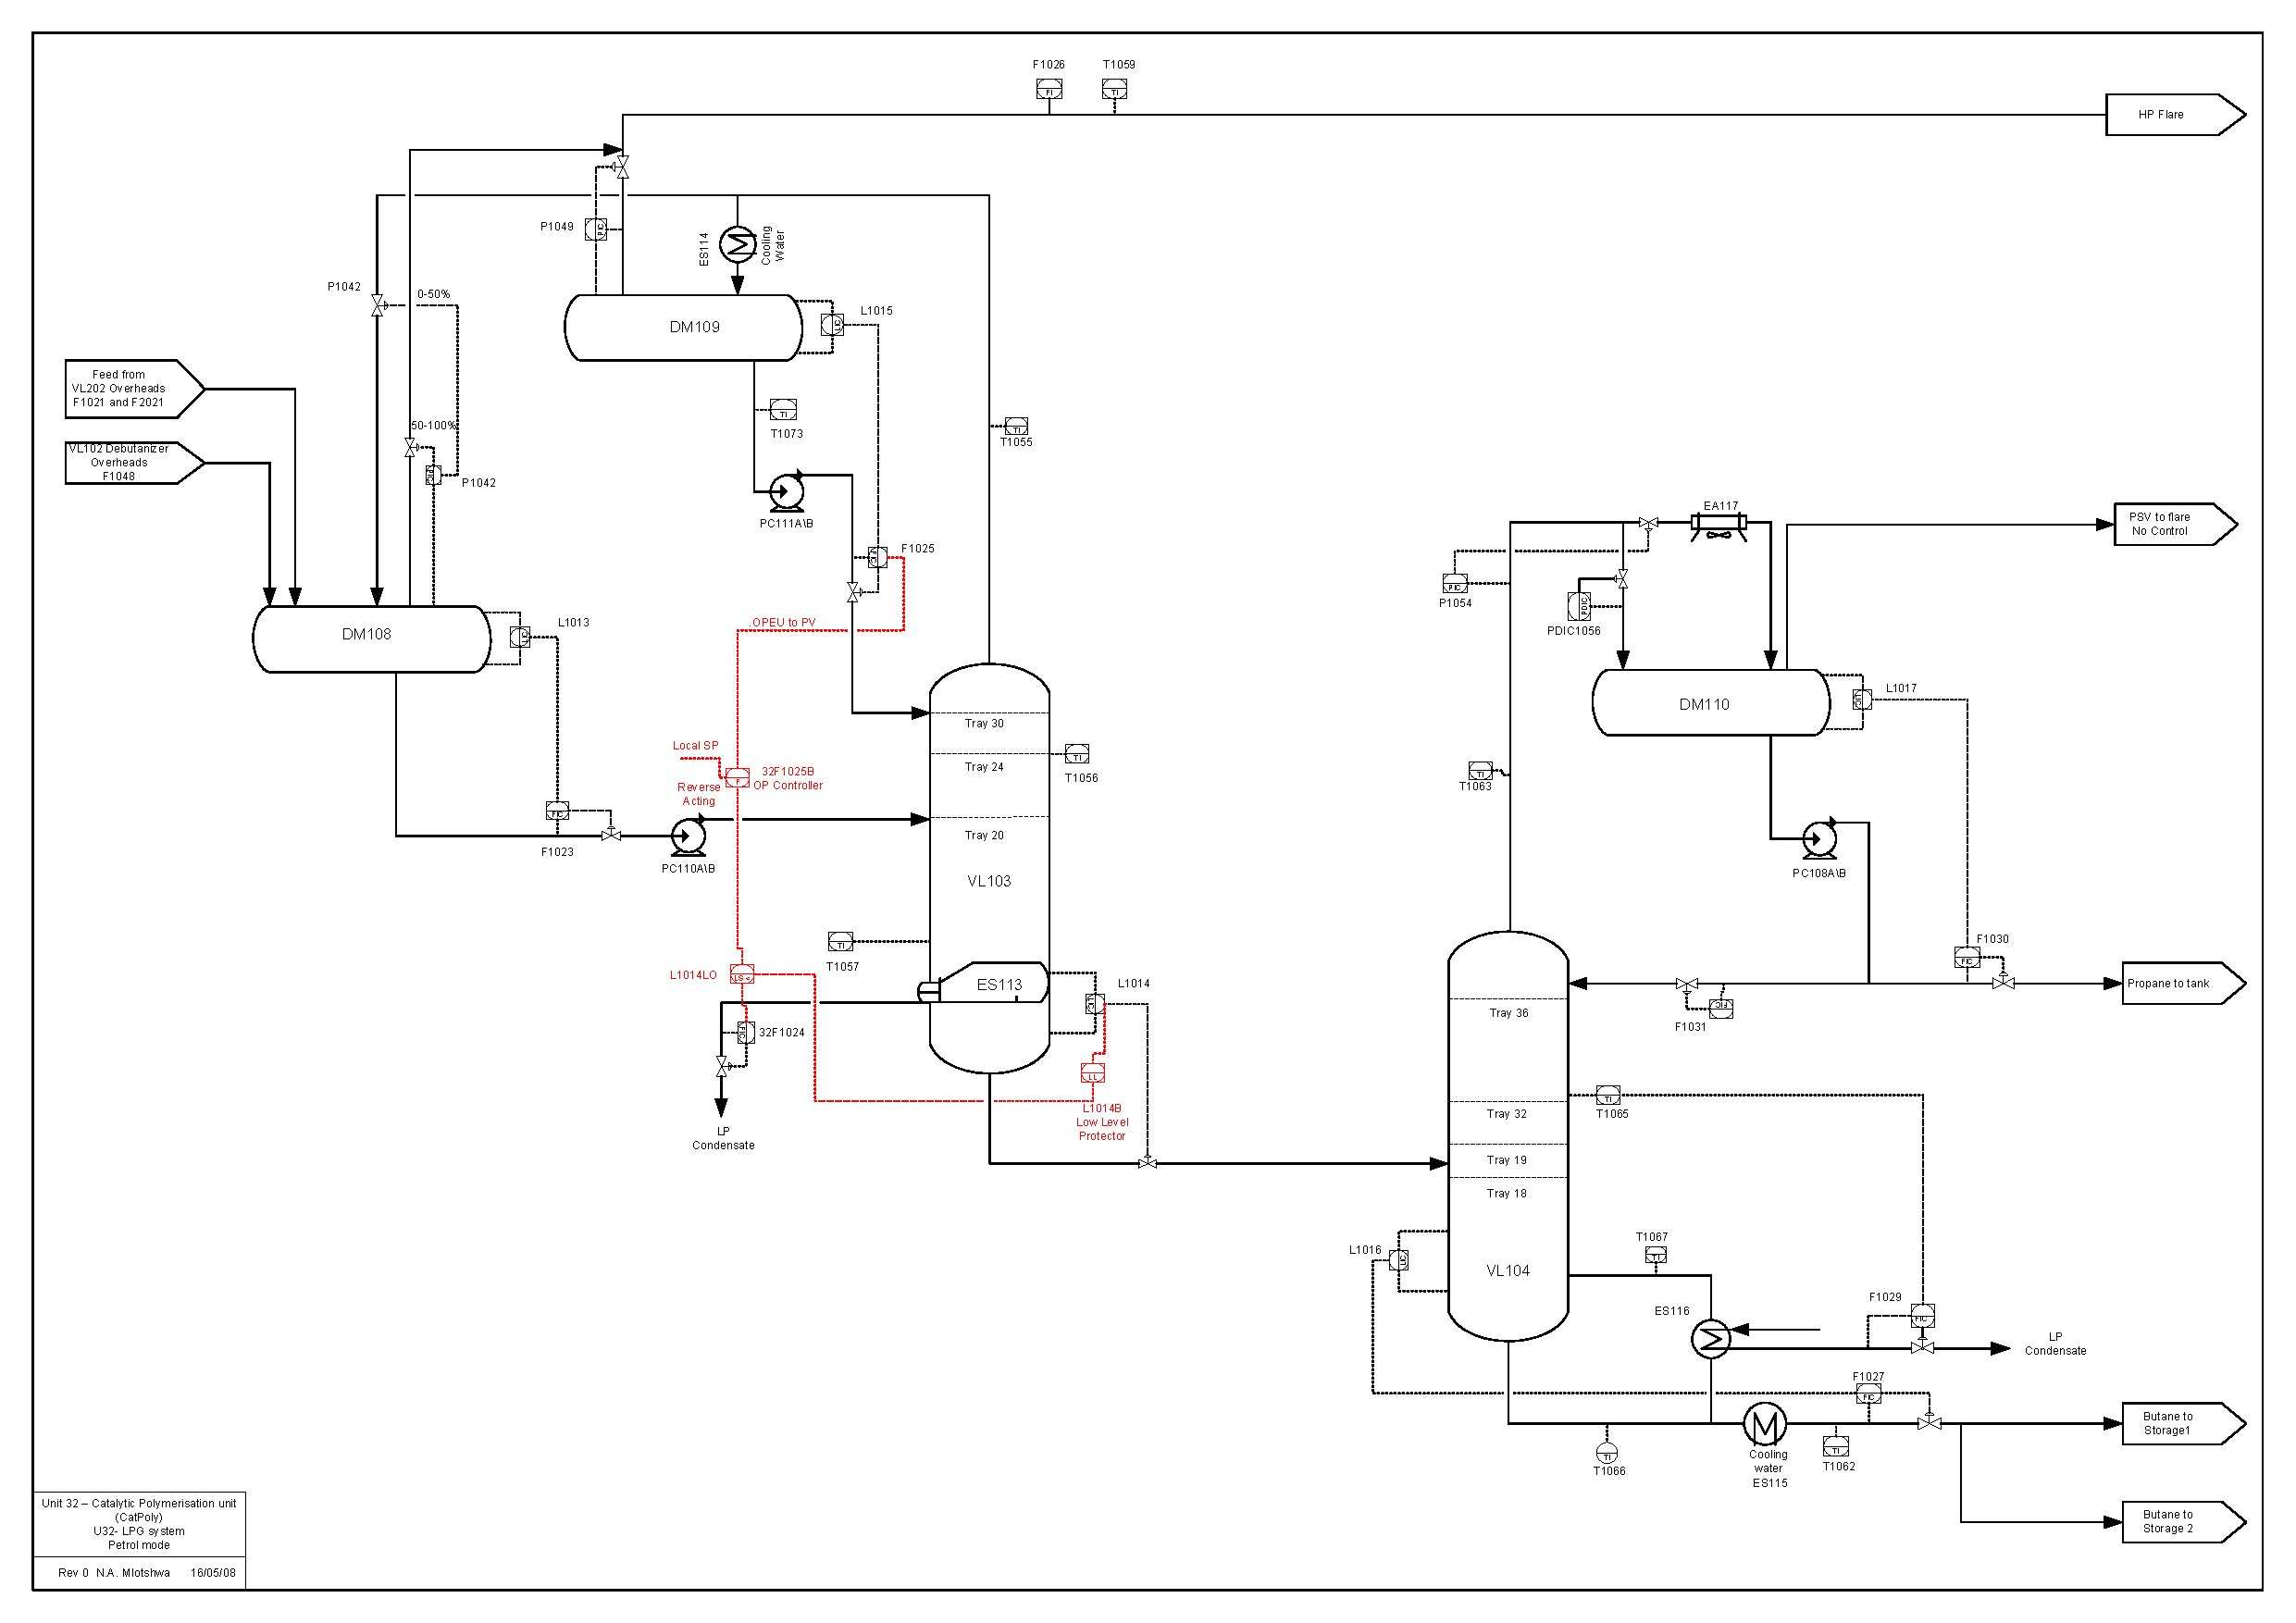
\includegraphics[width=\textwidth]{LPG_process}
  \caption[LPG process]{Industrial LPG process}
  \label{fig:lpgprocess}
\end{center}
\end{figure}

\section{Systems}
\subsection{Single tank}

\subsection{Two coupled tanks}
Allowing flow reversal

\subsection{Flash drum}

\subsection{Distillation column}

\subsection{Reactor}

\subsection{Reactor with flash drum and recycle}

\subsection{Tennessee Eastman challenge problem}
In 1993, \citet{downs.vogel1993plant-wide} proposed the Tennessee
Eastman plant-wide Industrial control problem as a test for new
control algorithms. The core of the process is a reactor with
a separation and recycle arrangement.  The flowsheet is shown in
Figure~\ref{fig:teprocess}.
\begin{figure}[htbp]
  \centering
  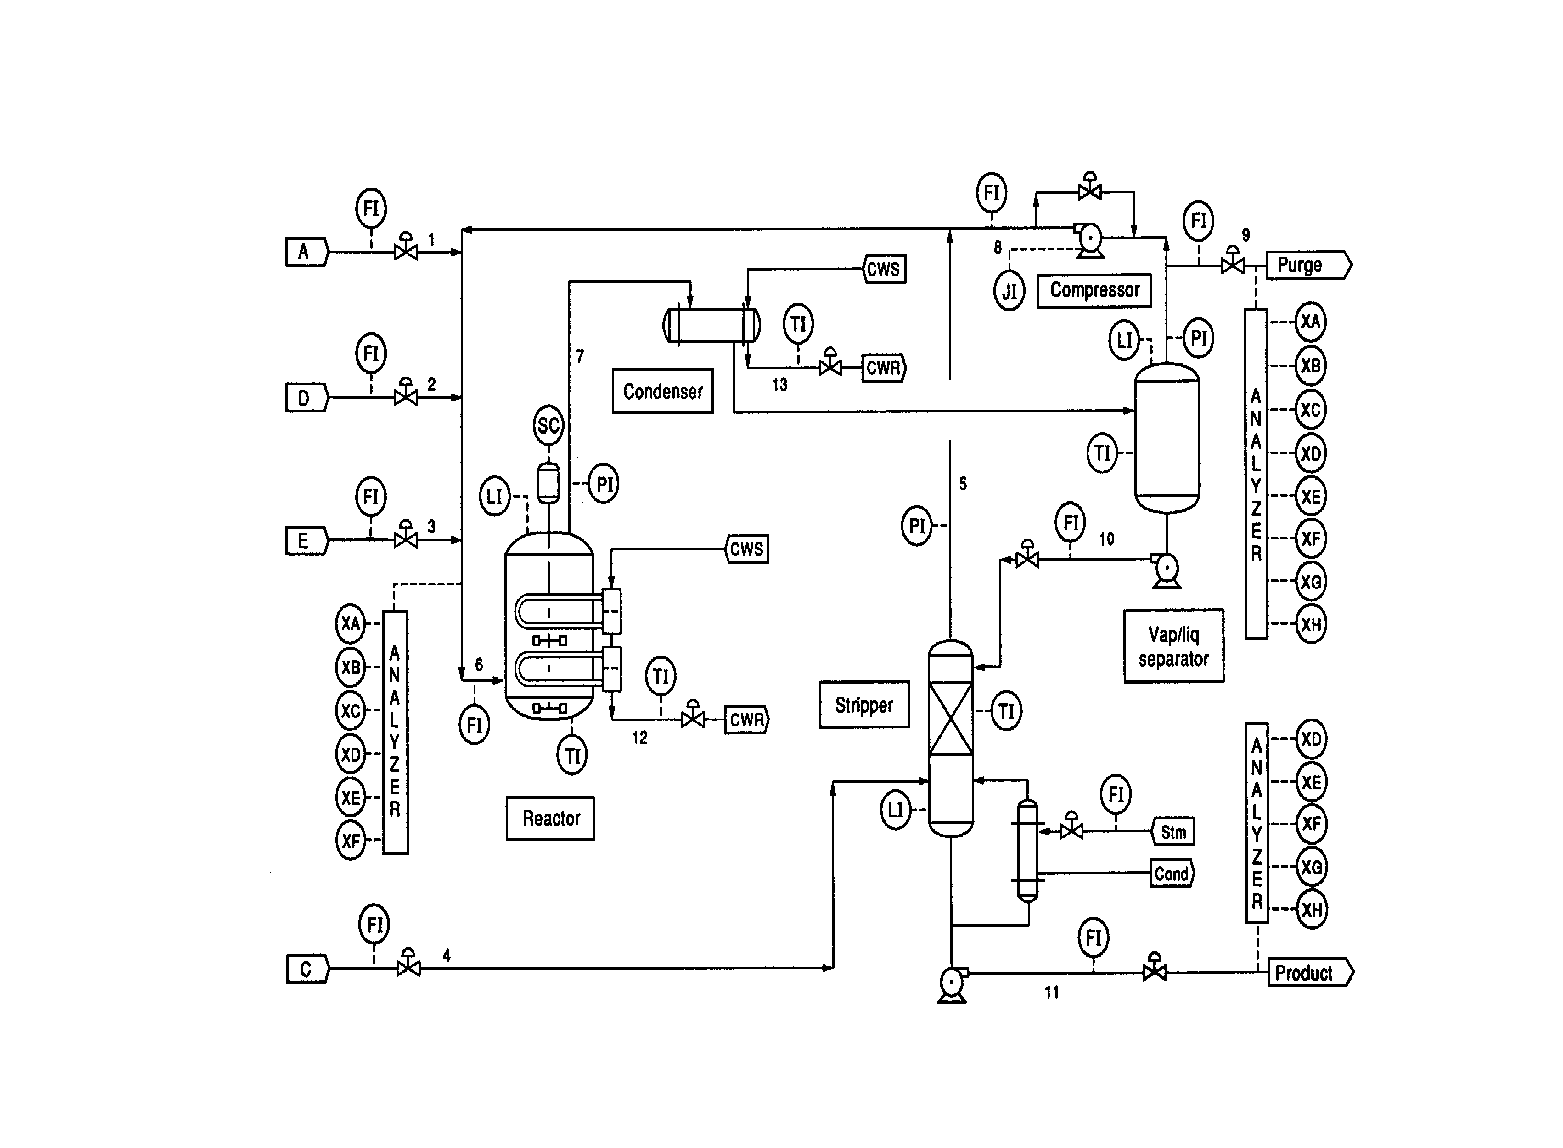
\includegraphics[width=\textwidth]{teflowsheet}
  \caption{Flowsheet for the Tennessee Eastman process~\citep{tenesseeeastman}}
  % TODO: Redraw TE flowsheet properly.
  \label{fig:teprocess}
\end{figure}

Four reactions featuring eight compounds (A through H) take place in the reactor:
\begin{eqnarray}
A(g) + C(g) + D(g) & \rightarrow & G(l) \\
A(g) + C(g) + E(g) & \rightarrow & H(l) \\
A(g) + E(g)        & \rightarrow & F(l) \\
3D(g)              & \rightarrow & 2F(l) 
\label{eq:te-reaction}
\end{eqnarray}

G and H are the first and second products, while F is a byproduct.

% Local Variables:
% TeX-master: "thesis"
% End:

